\documentclass{beamer}
\usepackage{scrextend}
\usepackage{amsfonts}
%\usepackage[T1]{fontenc}
\usepackage{booktabs}
\usepackage[latin1]{inputenc}
\usepackage{graphicx}
\usepackage{mathtools}
\usepackage{multimedia}
\usepackage{url}
\usetheme{Ilmenau}

\title[Monthly Meeting]{Inverse Procedural Generation of Geological Stories}
\author{Garcia Maxime}
%\institute{Mosig GVR}
%\date{January 2016}


\begin{document}

	
    \begin{frame}[label=(intro)]
	\titlepage
    \end{frame}
	
	
	\begin{frame}
	\frametitle{Today's agenda}
	\begin{itemize}
	\setbeamertemplate{itemize item}[ball]
	\item Simulation pipeline
	\setbeamertemplate{itemize item}[ball]
	\item Storytelling and geological events 
	\end{itemize}
	\end{frame}
	
	
	\section{Simulation Pipeline}
	
	\begin{frame}
	\frametitle{All Steps}
    \begin{itemize}
    \item Vec drawing analysis
    \item Story tree generation
    \item Simulation following one path of the tree
    \item Success evaluation
    \item Animation export in VAC
    \end{itemize}
    \end{frame}

	
    \begin{frame}
    \frametitle{Vec drawing analysis}
    \begin{itemize}
    \item Vec file input with color code
    \item Interlayers white colored
    \item Faults colored other than black or white
    %include chartreuse
    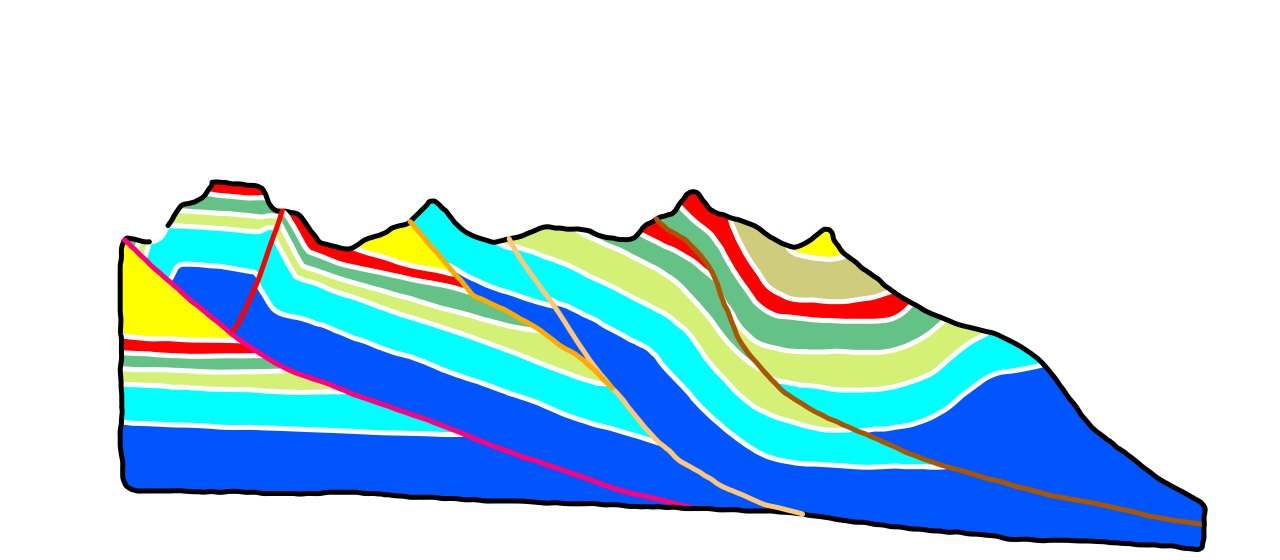
\includegraphics[scale=0.3]{chartreuse.png}
    \end{itemize}
    \end{frame}


	\begin{frame}
	\frametitle{Adding user information}
	\begin{itemize}
    \item Adding Material information
    %include screenshot material
    \item Adding Fault information
    %include screenshot fault
    \end{itemize}
	\end{frame}	


	\begin{frame}
	\frametitle{Automatic processing}
	\begin{itemize}
    \item Block structure detection
    \item Fault orientation
    \item Upper and lower blocks in fault (Compaction issue)
    %include compaction
    \item Output on a configuration file containing all the information (loosing vec info at the moment)
    \center{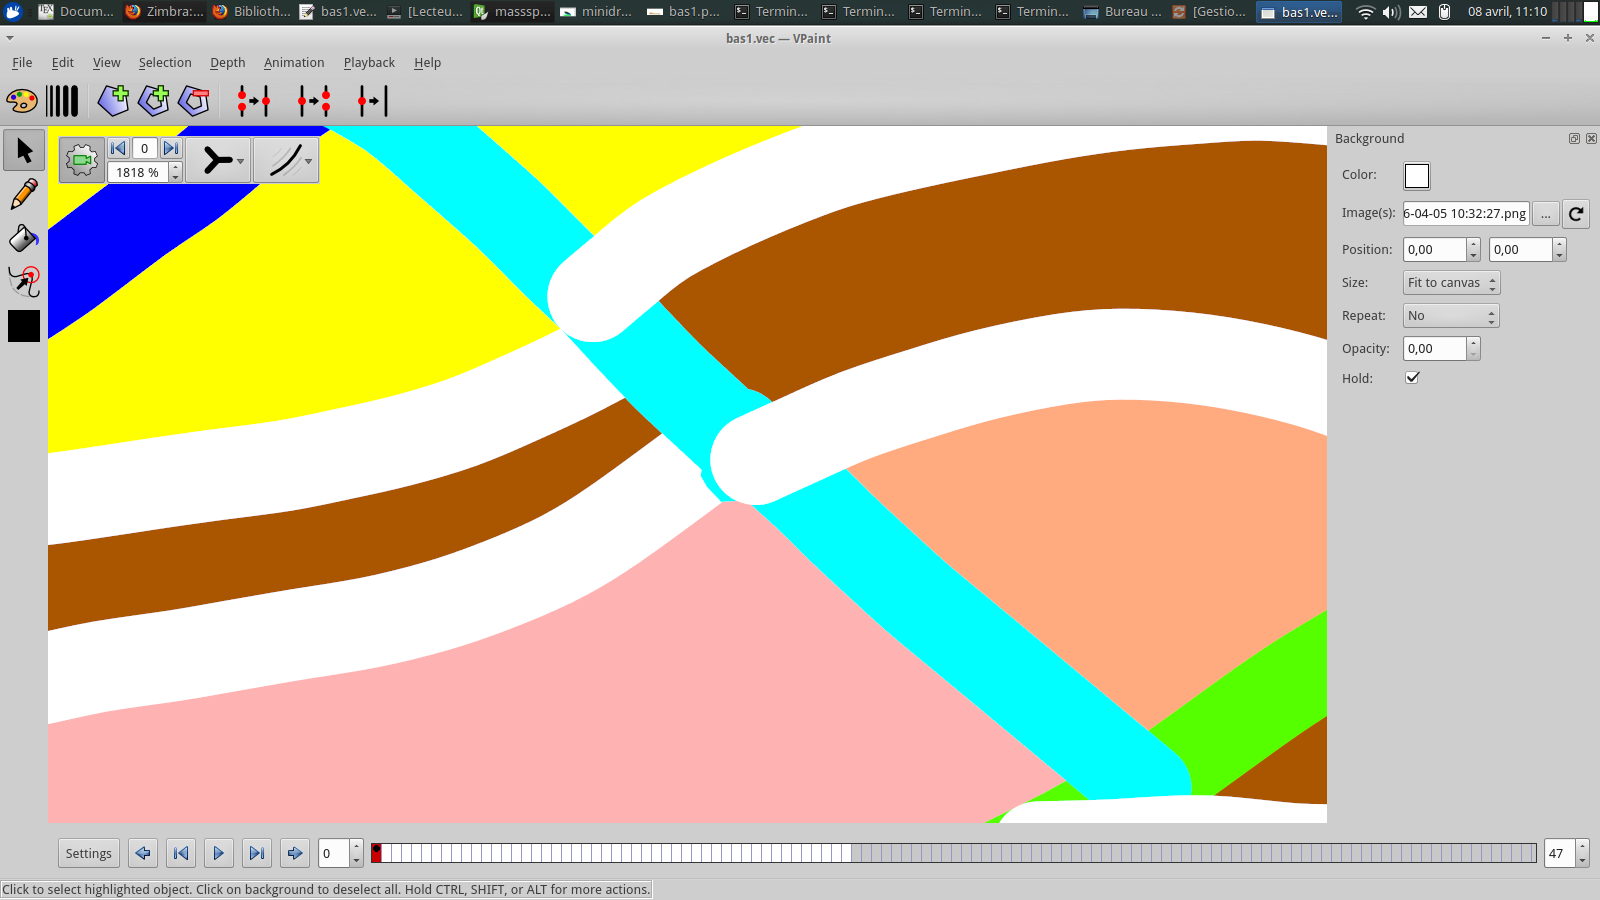
\includegraphics[scale=0.1]{compaction.png}}

    \end{itemize}
	\end{frame}	


	\begin{frame}
	\frametitle{Story Telling}
	\begin{itemize}
	\item Build a story tree with all possible event at one node
	\item Use user information to reduce the complexity
	\item Use automatic algo to reduce the complexity (Fault hierarchy for intance)
    \end{itemize}
	\end{frame}


	\begin{frame}
	\frametitle{Simulation/Animation}
	\begin{itemize}
	\item Choose one path in the tree
	\item For now just follow the user information for fault order.
	\item Generate Mass-Spring system for each layer of each block 
	\item Run the simulation with several input parameters. Several come from the configuration file (density, friction) and others are external but also configurable (dt, torsion, layer fusion condition, external forces)
	\end{itemize}
    \end{frame}


    \begin{frame} 
	\frametitle{Mass-Spring Genearation}
	\begin{itemize}
	\item Consider each layer being a quadrilateral having a width and height and build a mesh proportionnal to these two values (only width for now)
	\item Build the outline and use interpolation for the inside
	\item Sitck meshes if we have to (neighbouring layers)
	\item Block merging and recompute the mesh (optionnal)
	\end{itemize}
    \end{frame}
    
	
    \begin{frame} 
    \center{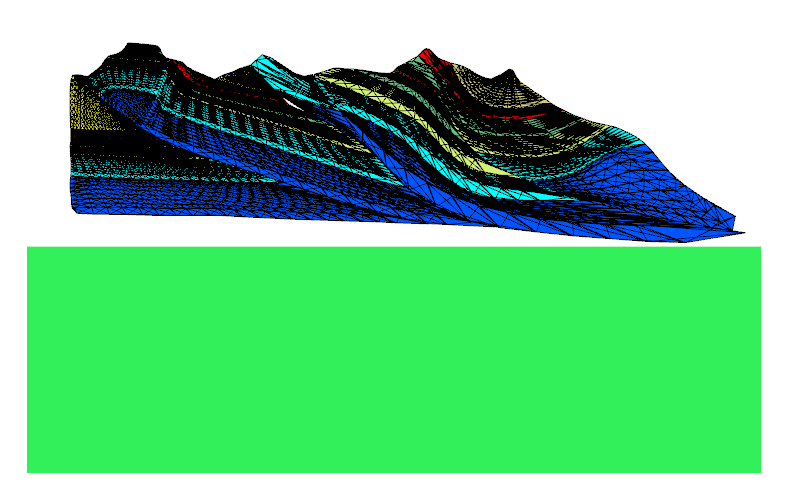
\includegraphics[scale=0.20]{chartreusespring.png}}
    \end{frame}   
    
    \begin{frame} 
    \frametitle{Simulation examples}
    %\movie[(autostart)]{}{(basBad.flv)}
    \url{basBad.flv}
    \\
    \url{miniChartreuseBad.flv}
    \end{frame}
	\section{Story Telling}
	
    \begin{frame}
    \frametitle{Principle}
    \begin{itemize}
    \item Build a tree of possible geological events at each node
    \item A branch is the animation of the selected events. Those events can make the simulation fail
    \item We can first provide the user a path where the simulation succed until there are no possible event to trigger.
    \item The user can choose to expand the tree by selecting other events at a precised node. 
    \end{itemize}
	\end{frame}
	
	\begin{frame}
	\frametitle{Detecting Event}
	\begin{itemize}
	\item Can we determine a local order (hierarchy) for faults ? 
	\item How can we detect and apply erosion ?
	\item How to simulate it ?
	\end{itemize}
	\end{frame}
	
            
\end{document}